\documentclass[10pt,aspectratio=169]{beamer}

\usetheme{metropolis}
\usepackage{appendixnumberbeamer}

\usepackage{booktabs}
\usepackage{tabularx}
\usepackage{multirow}
\usepackage{colortbl}
\usepackage{graphicx}
\usepackage{tikz}
\usepackage{pgfplots}
\pgfplotsset{compat=1.16}
\usetikzlibrary{shapes,arrows,positioning,calc}

\usepackage{amsmath}
\usepackage{amssymb}
\usepackage{pifont}

% Colors
\definecolor{winnergreen}{RGB}{39, 174, 96}
\definecolor{warningorange}{RGB}{230, 126, 34}
\definecolor{errorred}{RGB}{192, 57, 43}
\definecolor{niceblue}{RGB}{52, 152, 219}
\definecolor{lightgray}{RGB}{245, 245, 245}

\title{RRMC --- Week 6}
\subtitle{Scaling to 100 Puzzles \& Cross-Model Validation}
\date{2026-02-13}
\author{}
\institute{Qwen 2.5-7B + Gemma 3 27B via OpenRouter}

\begin{document}

\maketitle

%==============================================================================
\begin{frame}{What Changed This Week}
  \begin{columns}[T]
    \begin{column}{0.48\textwidth}
      \begin{block}{Scale \& Models}
        \begin{itemize}
          \item 20 $\rightarrow$ \textbf{100 puzzles} (all 3 tasks)
          \item Added \textbf{Gemma-3-27B} (cross-model)
          \item Tested Qwen3-Coder-30B-MoE on GN
        \end{itemize}
      \end{block}

      \vspace{0.3cm}

      \begin{block}{New Methods}
        \begin{itemize}
          \item \textbf{Zero-shot} baseline (0 turns)
          \item \textbf{MI-Only + min\_turns} guard
          \item min\_turns ablation (3, 5, 10)
        \end{itemize}
      \end{block}
    \end{column}

    \begin{column}{0.48\textwidth}
      \begin{alertblock}{Key Bug Fix}
        \texttt{\_clone\_stopping\_rule()} in the parallel evaluator
        dropped \texttt{min\_turns} when cloning MI stopping rules
        for threaded execution.

        \vspace{0.1cm}

        All MI experiments silently ran with \texttt{min\_turns=0}.
        Detected via GN showing avg turns = 1.1.
      \end{alertblock}

      \vspace{0.2cm}

      \textbf{Total:} 19 experiment runs, 3 tasks, 2 models, 8 methods
    \end{column}
  \end{columns}
\end{frame}

%==============================================================================
\section{Detective Cases (DC)}
%==============================================================================

\begin{frame}{DC Results: Qwen 7B (100 puzzles)}
  \begin{table}
    \centering
    \small
    \begin{tabular}{lccl}
      \toprule
      \textbf{Method} & \textbf{Accuracy} & \textbf{Avg Turns} & \textbf{Note} \\
      \midrule
      \rowcolor{winnergreen!15}
      KnowNo                & \textbf{41\%} & 1.0  & always stops T1 \\
      Zero-shot (T=0)       & 38\%          & 1.0  & no questions asked \\
      MI-Only (min3)        & 38\%          & 9.1  & = zero-shot at 9$\times$ turns \\
      CIP-Lite              & 37\%          & 1.3  & stops early \\
      Self-Consistency       & 34\%          & 1.5  & \\
      \midrule
      DQS + Fixed(10)       & 29\%          & 10.0 & \textcolor{errorred}{collapsed from 60\% at n=20} \\
      Fixed Turns (10)      & 25\%          & 10.0 & questioning hurts \\
      DQS + MI (min3)       & 24\%          & 8.9  & worst overall \\
      \bottomrule
    \end{tabular}
  \end{table}

  \vspace{0.2cm}

  \begin{columns}[T]
    \begin{column}{0.48\textwidth}
      \begin{alertblock}{DQS Collapse}
        n=20: 60\% $\rightarrow$ n=100: 29\%.

        The +30pp story was \textbf{lucky variance}.
      \end{alertblock}
    \end{column}
    \begin{column}{0.48\textwidth}
      \begin{exampleblock}{Zero-shot is the baseline}
        Zero-shot (38\%) $>$ Fixed(10) (25\%).

        Reading the case is better than investigating.
      \end{exampleblock}
    \end{column}
  \end{columns}
\end{frame}

\begin{frame}{DC: Why Questioning Hurts --- Puzzle 5}

  \small
  Ground truth: \textbf{Suspect D} \quad | \quad
  Zero-shot: \textcolor{winnergreen}{\textbf{D} \checkmark} \quad
  Fixed(10): \textcolor{errorred}{\textbf{E} \ding{55}}

  \vspace{0.2cm}

  \begin{columns}[T]
    \begin{column}{0.52\textwidth}
      \textbf{What happened during 10 turns of questioning:}

      \vspace{0.1cm}
      \footnotesize
      \begin{tabular}{rl}
        T1: & Clara Whitfield: ``I was at my usual cafe\ldots'' \\
        T4: & Victoria Blackwood: ``I was in my hotel room\ldots'' \\
        T5: & Eleanor Grey: ``I was in the library, locking up.'' \\
        T9: & Blackwood: ``Our disagreements were mostly academic\ldots'' \\
      \end{tabular}

      \normalsize
      \vspace{0.3cm}

      Every suspect gave \textbf{plausible alibis} and \textbf{denied conflicts}.
      The model was confused by uniform denials
      $\rightarrow$ \textbf{switched} from correct D to wrong E.
    \end{column}

    \begin{column}{0.44\textwidth}
      \begin{alertblock}{The Pattern (24 puzzles)}
        Model starts with correct intuition from case description.

        \vspace{0.1cm}

        Asks uninformative questions $\rightarrow$ generic alibis
        $\rightarrow$ model \textbf{second-guesses itself}
        $\rightarrow$ switches to wrong answer.
      \end{alertblock}

      \vspace{0.2cm}

      \begin{block}{Disagreement Counts}
        \footnotesize
        \begin{tabular}{lc}
          Zero-shot \checkmark, Fixed(10) \ding{55} & \textbf{24} \\
          Zero-shot \ding{55}, Fixed(10) \checkmark & 11 \\
          Both correct & 14 \\
          Both wrong & 51 \\
        \end{tabular}

        Net: $-$13 puzzles from questioning.
      \end{block}
    \end{column}
  \end{columns}
\end{frame}

\begin{frame}{DC: A Directly Answerable Case --- Puzzle 17}

  \small
  Victim: \textbf{Jonathan Blake} (architect) \quad
  Weapon: \textbf{blood-stained sculpture piece} \quad
  Zero-shot: \textcolor{winnergreen}{\textbf{A} \checkmark} \quad
  Fixed(10): \textcolor{errorred}{\textbf{E} \ding{55}}

  \vspace{0.1cm}

  \begin{columns}[T]
    \begin{column}{0.48\textwidth}
      \textbf{Case description already answers it:}

      \vspace{0.05cm}
      \footnotesize
      \begin{tabular}{cl}
        \textbf{A:} & \textbf{Eleanor Whitaker} --- artist known for \\
                     & \textbf{avant-garde sculptures}, ``fiercely \\
                     & competitive, public disagreements'' \\[3pt]
        B: & Sophia Carter --- art curator \\[1pt]
        C: & Michael Turner --- real estate developer \\[1pt]
        D: & Clara Mitchell --- landscape architect \\[1pt]
        E: & Oliver Bennett --- park worker (found body) \\
      \end{tabular}

      \normalsize
      \vspace{0.1cm}

      Murder weapon = \textbf{sculpture}.
      Only one suspect makes sculptures.
      Zero-shot sees this immediately.
    \end{column}

    \begin{column}{0.48\textwidth}
      \textbf{What 10 turns of questioning did:}

      \footnotesize
      \vspace{0.05cm}
      \begin{tabular}{rp{5cm}}
        T1: & Whitaker: ``interactions were always tense'' \\[1pt]
        T4: & Whitaker: ``sculpture was central to my installation'' \\[1pt]
        T8: & Bennett: ``someone had been fiddling with it'' \\[1pt]
        T9: & Whitaker: ``blood-stained when Jonathan accidentally\ldots'' \\
      \end{tabular}

      \normalsize
      \vspace{0.1cm}

      \begin{alertblock}{Questioning Obscured the Signal}
        Whitaker deflected (``accidentally'').
        Bennett's proximity to body $\rightarrow$ looked suspicious.
        Model switched A $\rightarrow$ E.

        \textbf{Solvable from the description alone.}
      \end{alertblock}
    \end{column}
  \end{columns}
\end{frame}

\begin{frame}{DC: When Questioning Helps --- Puzzle 3}

  \small
  Ground truth: \textbf{E / Alex Turner} \quad | \quad
  Zero-shot: \textcolor{errorred}{\textbf{D} \ding{55}} \quad
  Fixed(10): \textcolor{winnergreen}{\textbf{E} \checkmark}

  \vspace{0.2cm}

  \begin{columns}[T]
    \begin{column}{0.52\textwidth}
      \textbf{Key turns:}

      \vspace{0.1cm}
      \footnotesize
      \begin{tabular}{rl}
        T5: & Alex Turner: ``I was setting up for a freelance \\
            & project meeting, but it didn't go as planned.'' \\[3pt]
        T9: & Turner: ``Yes, we had some disagreements about \\
            & the direction of the project\ldots'' \\
      \end{tabular}

      \normalsize
      \vspace{0.2cm}

      Meanwhile, all other suspects denied conflicts:
      \begin{itemize}
        \footnotesize
        \item Reynolds: ``No, I had no disputes''
        \item Davis: ``No, I don't think so''
        \item Mitchell: ``No, I did not have any disputes''
      \end{itemize}

      \normalsize
      Turner's admission stood out $\rightarrow$ model corrected to E.
    \end{column}

    \begin{column}{0.44\textwidth}
      \begin{exampleblock}{Success Pattern (11 puzzles)}
        The guilty suspect \textbf{admits to conflicts} or suspicious behavior
        while innocents uniformly deny.

        \vspace{0.1cm}

        This contrast gives the model a clear signal --- but it only works
        \textbf{11 out of 100 times}.
      \end{exampleblock}

      \vspace{0.2cm}

      \begin{block}{Takeaway}
        Questioning helps only when NPCs
        \textbf{differentially leak guilt}.

        \vspace{0.1cm}

        Most of the time, all suspects give the same
        generic alibis $\rightarrow$ noise.
      \end{block}
    \end{column}
  \end{columns}
\end{frame}

%==============================================================================
\begin{frame}{DC Cross-Model: Gemma 27B (100 puzzles)}
  \begin{table}
    \centering
    \begin{tabular}{lccc}
      \toprule
      \textbf{Method} & \textbf{Gemma-3-27B} & \textbf{Qwen-2.5-7B} & \textbf{$\Delta$} \\
      \midrule
      \rowcolor{winnergreen!15}
      Zero-shot     & \textbf{57\%}  & 38\% & \textcolor{winnergreen}{$+$19pp} \\
      Fixed(10)     & 40\%           & 25\% & $+$15pp \\
      DQS+Fixed(10) & 30\%           & 29\% & $+$1pp \\
      \bottomrule
    \end{tabular}
  \end{table}

  \vspace{0.3cm}

  \begin{columns}[T]
    \begin{column}{0.48\textwidth}
      \begin{exampleblock}{Model Scale Dominates}
        Gemma-27B zero-shot (\textbf{57\%}) gains more from scale ($+$19pp)
        than any method ever achieved.

        \vspace{0.1cm}

        No stopping rule or DQS comes close.
      \end{exampleblock}
    \end{column}
    \begin{column}{0.48\textwidth}
      \begin{alertblock}{Questioning Hurts More with 27B}
        27B: 57\% $\rightarrow$ 40\% (\textcolor{errorred}{$-$17pp})

        7B: 38\% $\rightarrow$ 25\% (\textcolor{errorred}{$-$13pp})

        \vspace{0.1cm}

        DQS hurts 27B further: 40\% $\rightarrow$ 30\% (\textcolor{errorred}{$-$10pp}).

        \vspace{0.1cm}

        \textbf{Task-inherent}, not model-specific.
      \end{alertblock}
    \end{column}
  \end{columns}
\end{frame}

\begin{frame}{DC: Why DQS Hurts the Stronger Model --- Puzzle 40}

  \small
  Ground truth: \textbf{E} \quad | \quad
  Zero-shot: \textcolor{winnergreen}{\textbf{E} \checkmark} \quad
  Fixed(10): \textcolor{winnergreen}{\textbf{E} \checkmark} \quad
  DQS: \textcolor{errorred}{\textbf{D} \ding{55}}

  \vspace{0.2cm}

  \begin{columns}[T]
    \begin{column}{0.48\textwidth}
      \textbf{Fixed(10)} --- simple, focused questions:

      \footnotesize
      ``What were you doing between 9pm and 10pm?''

      \normalsize
      \vspace{0.1cm}
      Systematically covered each suspect.
      Answers naturally revealed useful patterns.

      \vspace{0.3cm}

      \textbf{DQS} --- elaborate, leading questions:

      \footnotesize
      ``Given your reputation for dealing in valuable art
      and your close ties to Eleanor, can you provide any insight
      into why someone would want to harm her\ldots?''

      \normalsize
      \vspace{0.1cm}
      Suspects gave longer, more \textbf{evasive} non-answers.
    \end{column}

    \begin{column}{0.48\textwidth}
      \begin{alertblock}{DQS Failure Modes}
        \begin{enumerate}
          \item \textbf{Leading questions} telegraph suspicion
                $\rightarrow$ evasive answers
          \item \textbf{Fixation}: DQS asked one suspect 4/9 turns,
                creating an echo chamber
          \item \textbf{Complexity}: compound questions
                generate compound non-answers
        \end{enumerate}
      \end{alertblock}

      \vspace{0.2cm}

      \begin{block}{10 ``easy'' puzzles broken}
        \footnotesize
        Both zero-shot AND Fixed(10) correct,
        but DQS still got wrong.

        DQS introduces noise even on easy puzzles.
      \end{block}
    \end{column}
  \end{columns}
\end{frame}

%==============================================================================
\section{Situation Puzzles (SP)}
%==============================================================================

\begin{frame}{SP Results: Qwen 7B (100 puzzles)}
  \begin{table}
    \centering
    \begin{tabular}{lcccc}
      \toprule
      \textbf{Method} & \textbf{Bool Acc} & \textbf{Avg F1 (char)} & \textbf{Avg Turns} & \textbf{Note} \\
      \midrule
      \rowcolor{winnergreen!15}
      \textbf{MI-Only (min3)} & 99\% & \textbf{0.799} & 3.0 & best F1, $p < 0.001$ \\
      Zero-shot              & 100\% & 0.719           & 1.0 & baseline \\
      CIP-Lite               & 100\% & 0.718           & 1.5 & $\approx$ zero-shot \\
      Fixed Turns (10)       & 100\% & 0.716           & 10.0 & 10 turns, no F1 gain \\
      \bottomrule
    \end{tabular}
  \end{table}

  \vspace{0.3cm}

  \begin{columns}[T]
    \begin{column}{0.48\textwidth}
      \begin{exampleblock}{MI's One Clean Win}
        F1: 0.72 $\rightarrow$ \textbf{0.80} ($+$0.08, paired $t$-test $p < 0.001$).

        \vspace{0.1cm}

        MI-Only(min3) outperforms on \textbf{69/100} puzzles.
        The only task where MI-based stopping genuinely helps.
      \end{exampleblock}
    \end{column}
    \begin{column}{0.48\textwidth}
      \begin{alertblock}{Boolean Acc is Uninformative}
        All methods score 99--100\%.

        Character-level F1 is the \textbf{only} metric
        that differentiates methods.

        \vspace{0.1cm}

        Generic questions don't help: Fixed(10) $\approx$ zero-shot.
      \end{alertblock}
    \end{column}
  \end{columns}
\end{frame}

\begin{frame}{SP: Why MI Works --- Puzzle 53}

  \small
  \textbf{Puzzle:} ``Sarah is seen in two places at once. How?''

  Ground truth: \textit{Sarah has an identical twin who covers for her.}

  \vspace{0.1cm}

  Zero-shot F1: 0.168 \quad | \quad MI-Only F1: \textbf{0.333} ($+$0.165)

  \vspace{0.2cm}

  \begin{columns}[T]
    \begin{column}{0.52\textwidth}
      \textbf{MI-Only Q\&A (stopped at turn 4):}

      \vspace{0.1cm}
      \footnotesize
      \begin{tabular}{rp{6cm}}
        T1: & Q: Technology to appear in two places? \\
            & A: \textbf{No} \quad {\color{gray}(MI=0.45 --- high uncertainty)} \\[3pt]
        T2: & Q: Remote working setup? \\
            & A: \textbf{No} \quad {\color{gray}(MI=0.0)} \\[3pt]
        T3: & Q: Does she have a \textbf{double}? \\
            & A: \textbf{Yes} \quad {\color{gray}(MI=0.45 --- still uncertain)} \\[3pt]
        T4: & \textit{(stopped --- MI=0.0, converged)} \\
      \end{tabular}

      \normalsize
      \vspace{0.2cm}

      Prediction: ``Sarah has a \textbf{twin sister}\ldots''
    \end{column}

    \begin{column}{0.44\textwidth}
      \textbf{Zero-shot} (no questions):

      \vspace{0.1cm}

      ``Sarah might be using \textbf{virtual reality}
      or advanced telepresence technology\ldots''

      \vspace{0.3cm}

      \begin{exampleblock}{Why It Works}
        Yes/no feedback is \textbf{ground-truth} ---
        not LLM-generated noise.

        \vspace{0.1cm}

        T1--T2 \textbf{eliminated} technology hypotheses.

        T3 \textbf{confirmed} the ``double'' direction.

        \vspace{0.1cm}

        Systematic elimination $\rightarrow$ correct answer.
      \end{exampleblock}
    \end{column}
  \end{columns}
\end{frame}

\begin{frame}{SP: When MI Hurts --- Puzzle 48}

  \small
  \textbf{Puzzle:} ``John has never left his hometown, yet seen in two countries. How?''
  \quad Ground truth: \textit{Identical twin + video calls.}

  \vspace{0.05cm}

  Zero-shot F1: \textbf{0.377} \quad | \quad MI-Only F1: 0.216 ($-$0.161)

  \vspace{0.15cm}

  \begin{columns}[T]
    \begin{column}{0.52\textwidth}
      \textbf{MI-Only Q\&A:}

      \vspace{0.1cm}
      \footnotesize
      \begin{tabular}{rp{6cm}}
        T1: & Q: Does John use technology to appear in both? \\
            & A: \textbf{No} \quad {\color{errorred}(misleading --- video calls ARE technology)} \\[3pt]
        T2: & Q: Did John travel at different times? \\
            & A: \textbf{No} \\
      \end{tabular}

      \normalsize
      \vspace{0.15cm}

      Model \textbf{ruled out technology} based on misleading ``No''
      $\rightarrow$ guessed ``conspiracy or hoax.''

      \vspace{0.15cm}

      \textbf{Zero-shot:} guessed ``hologram / projection'' ---
      closer to video calls $\rightarrow$ higher F1.
    \end{column}

    \begin{column}{0.44\textwidth}
      \begin{alertblock}{Failure Mode}
        SP uses an LLM referee for yes/no answers.

        \vspace{0.05cm}

        Referee answered ``No'' to a technology question
        when the ground truth \textbf{involves} technology (video calls).

        \vspace{0.05cm}

        Misleading feedback \textbf{poisoned} the reasoning ---
        model ruled out the correct direction.
      \end{alertblock}

      \vspace{0.15cm}

      \begin{block}{Net Result}
        MI better on \textbf{69} puzzles, worse on \textbf{29}.
        Referee quality limits the ceiling.
      \end{block}
    \end{column}
  \end{columns}
\end{frame}

%==============================================================================
\section{Guessing Numbers (GN)}
%==============================================================================

\begin{frame}{GN Results: Gemma 27B (100 puzzles)}
  \begin{table}
    \centering
    \begin{tabular}{lccc}
      \toprule
      \textbf{Method} & \textbf{Accuracy} & \textbf{Avg Turns} & \textbf{Note} \\
      \midrule
      \textit{Algorithmic DQS} & \textit{100\%} & \textit{5.4} & \textit{not LLM} \\
      \midrule
      \rowcolor{winnergreen!15}
      \textbf{Fixed(25)}    & \textbf{12\%} & 23.8 & best LLM method \\
      MI-Only (min10)       & 9\%           & 17.5 & \\
      DQS + Fixed(25)       & 4\%           & 24.5 & \textcolor{errorred}{DQS hurts again} \\
      MI-Only (min5)        & 2\%           & 8.8  & stops too early \\
      MI-Only (min3)        & 1\%           & 6.1  & way too early \\
      Self-Consistency       & 0\%           & 2.8  & immediate wrong stop \\
      \midrule
      \textit{Qwen 7B (any method)} & \textit{0\%} & --- & \textit{model too weak} \\
      \textit{Qwen3-Coder-30B-MoE} & \textit{0\%} & --- & \textit{3B active = too weak} \\
      \bottomrule
    \end{tabular}
  \end{table}

  \vspace{0.2cm}

  \begin{exampleblock}{}
    \textbf{First non-zero LLM result on GN.} Dense 27B breaks the 0\% barrier.
    Model needs \textbf{maximum turns} --- any early stopping hurts.
  \end{exampleblock}
\end{frame}

\begin{frame}{GN: min\_turns Ablation}

  \begin{columns}[T]
    \begin{column}{0.45\textwidth}
      \begin{center}
      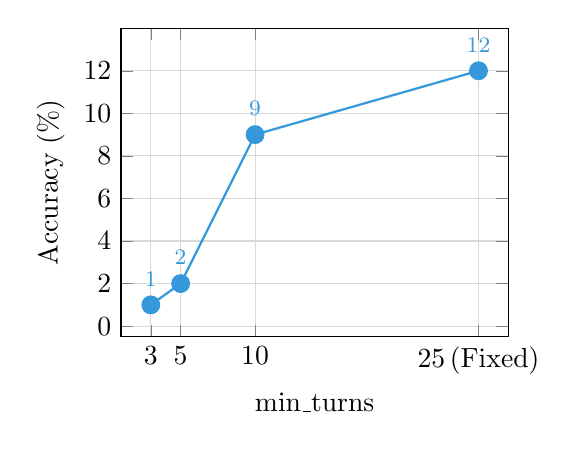
\begin{tikzpicture}
        \begin{axis}[
          width=6.5cm, height=5.5cm,
          xlabel={min\_turns},
          ylabel={Accuracy (\%)},
          xtick={3,5,10,25},
          xticklabels={3,5,10,25\,(Fixed)},
          ytick={0,2,4,6,8,10,12},
          ymin=-0.5, ymax=14,
          xmin=1, xmax=27,
          grid=major,
          grid style={gray!30},
          mark size=3pt,
          nodes near coords,
          every node near coord/.append style={font=\footnotesize, above=3pt},
        ]
          \addplot[thick, mark=*, niceblue] coordinates {
            (3, 1) (5, 2) (10, 9) (25, 12)
          };
        \end{axis}
      \end{tikzpicture}
      \end{center}
    \end{column}

    \begin{column}{0.52\textwidth}
      \begin{block}{Clear Monotonic Trend}
        More investigation turns $=$ higher accuracy.

        \vspace{0.1cm}

        \begin{tabular}{lcc}
          \toprule
          \textbf{min\_turns} & \textbf{Acc} & \textbf{Avg Turns} \\
          \midrule
          3 & 1\% & 6.1 \\
          5 & 2\% & 8.8 \\
          10 & 9\% & 17.5 \\
          25 (Fixed) & \textbf{12\%} & 23.8 \\
          \bottomrule
        \end{tabular}
      \end{block}

      \vspace{0.2cm}

      \begin{alertblock}{MI Stopping is Wrong for GN}
        MI detects ``convergence'' but the model converges on
        \textbf{wrong answers}.

        \vspace{0.1cm}

        GN needs all available evidence before answering.
        Early stopping = premature commitment.
      \end{alertblock}
    \end{column}
  \end{columns}
\end{frame}

\begin{frame}{GN: What Gemma Does Right --- Puzzle 51 (Solved in 4 turns)}

  \small
  Secret: \textbf{5670}

  \vspace{0.2cm}

  \begin{columns}[T]
    \begin{column}{0.48\textwidth}
      \footnotesize
      \begin{tabular}{rccl}
        \toprule
        \textbf{Turn} & \textbf{Guess} & \textbf{Feedback} & \textbf{Reasoning} \\
        \midrule
        1 & 1234 & 0B 0C & eliminates 1,2,3,4 \\
        2 & 5678 & 3B 0C & 3 of \{5,6,7,8\} in position \\
        3 & 5679 & 3B 0C & swapped 8$\rightarrow$9: same 3B \\
          &      &       & $\Rightarrow$ 8 \textit{and} 9 not at pos 4 \\
          &      &       & $\Rightarrow$ pos 4 must be 0 \\
        \midrule
        \rowcolor{winnergreen!15}
        4 & \textbf{5670} & \textbf{4B} & \textcolor{winnergreen}{\textbf{Correct!}} \\
        \bottomrule
      \end{tabular}

      \normalsize
      \vspace{0.3cm}

      \textbf{Perfect deduction:}
      T1 eliminates half the digits.
      T2 finds 3 bulls.
      T3 tests the remaining position.
      T4 fills in the only possibility.
    \end{column}

    \begin{column}{0.48\textwidth}
      \begin{exampleblock}{Solve Distribution (12/100)}
        \footnotesize
        \begin{tabular}{lc}
          \toprule
          \textbf{Category} & \textbf{Count} \\
          \midrule
          Early ($<$15 turns) & 6 \\
          Late (15--25 turns) & 6 \\
          \midrule
          Fastest & 4 turns (idx=51) \\
          Slowest & 24 turns (idx=93) \\
          \bottomrule
        \end{tabular}

        \normalsize
        \vspace{0.2cm}

        Even split between fast solvers (clean deduction)
        and slow solvers (stumble into the answer).
      \end{exampleblock}
    \end{column}
  \end{columns}
\end{frame}

\begin{frame}{GN: The ``Last Mile'' Problem --- Puzzle 56 (3 Bulls, 5 Times, Never Solved)}

  \small
  Secret: \textbf{6728} \quad | \quad Result: \textcolor{errorred}{\textbf{Wrong}} (predicted 6718)

  \vspace{0.2cm}

  \begin{columns}[T]
    \begin{column}{0.52\textwidth}
      \footnotesize
      \begin{tabular}{rccl}
        \toprule
        \textbf{Turn} & \textbf{Guess} & \textbf{Result} & \\
        \midrule
        14 & 67\textbf{2}3 & \textbf{3B} 0C & pos 1,2,3 correct! \\
        \rowcolor{errorred!10}
        15 & 6745 & 2B 0C & \textit{abandoned pos 3!} \\
        18 & 6738 & 3B 0C & found 67\_8 \\
        22 & 6729 & 3B 0C & tried 9 at pos 4 \\
        23 & 6708 & 3B 0C & tried 0 at pos 3 \\
        24 & 6718 & 3B 0C & tried 1 at pos 3 \\
        \bottomrule
      \end{tabular}

      \normalsize
      \vspace{0.2cm}

      Turn 14 had \texttt{672\_} --- only needed to try
      digits at position 4.

      But the model \textbf{abandoned} the correct `2' at pos 3
      and \textbf{never returned to it}.
    \end{column}

    \begin{column}{0.44\textwidth}
      \begin{alertblock}{No Constraint Memory}
        The model doesn't maintain a record of
        ``which positions are proven correct.''

        \vspace{0.1cm}

        After finding \texttt{67\_\_}, it tried
        \texttt{6738}, \texttt{6729}, \texttt{6708}, \texttt{6718}
        --- systematically \textbf{avoiding} the correct
        \texttt{672\_} prefix.
      \end{alertblock}

      \vspace{0.2cm}

      \begin{block}{Scale of the Problem}
        \textbf{31 of 88} failed puzzles reached 3 bulls
        at some point but couldn't close.

        \vspace{0.1cm}

        Avg first 3-bull hit: turn 14.6.

        The model \textbf{can} narrow to 3/4 digits
        but cannot \textbf{systematically} test the last one.
      \end{block}
    \end{column}
  \end{columns}
\end{frame}

%==============================================================================
\section{Cross-Task Summary}
%==============================================================================

\begin{frame}{Cross-Task Summary}
  \begin{table}
    \centering
    \small
    \begin{tabular}{lcccc}
      \toprule
      & \textbf{DC (7B)} & \textbf{DC (27B)} & \textbf{SP (7B)} & \textbf{GN (27B)} \\
      \midrule
      Best LLM method
        & KnowNo 41\%
        & Zero-shot \textbf{57\%}
        & MI-Only \textbf{F1=0.80}
        & Fixed(25) 12\% \\[3pt]
      Questioning helps?
        & \textcolor{errorred}{No ($-$13pp)}
        & \textcolor{errorred}{No ($-$17pp)}
        & \textcolor{winnergreen}{Yes ($+$0.08)}
        & \textcolor{winnergreen}{Yes ($+$12pp)} \\[3pt]
      DQS helps?
        & \textcolor{errorred}{No}
        & \textcolor{errorred}{$-$10pp}
        & ---
        & \textcolor{errorred}{$-$8pp} \\[3pt]
      MI stopping helps?
        & \textcolor{errorred}{No}
        & ---
        & \textcolor{winnergreen}{Yes}
        & \textcolor{errorred}{No} \\[3pt]
      Best strategy
        & Stop T1
        & Stop T1
        & Stop T3
        & Use all 25 \\
      \bottomrule
    \end{tabular}
  \end{table}

  \vspace{0.3cm}

  \begin{exampleblock}{The Critical Factor: Feedback Quality}
    \textbf{DC:} LLM-generated NPC responses = \textcolor{errorred}{noise}.
    \textbf{SP:} Ground-truth yes/no = \textcolor{winnergreen}{signal}.
    \textbf{GN:} Precise constraints = \textcolor{winnergreen}{signal} (but needs strong model to exploit).
  \end{exampleblock}
\end{frame}

\begin{frame}{DQS: A Universal Negative Result}

  \begin{center}
  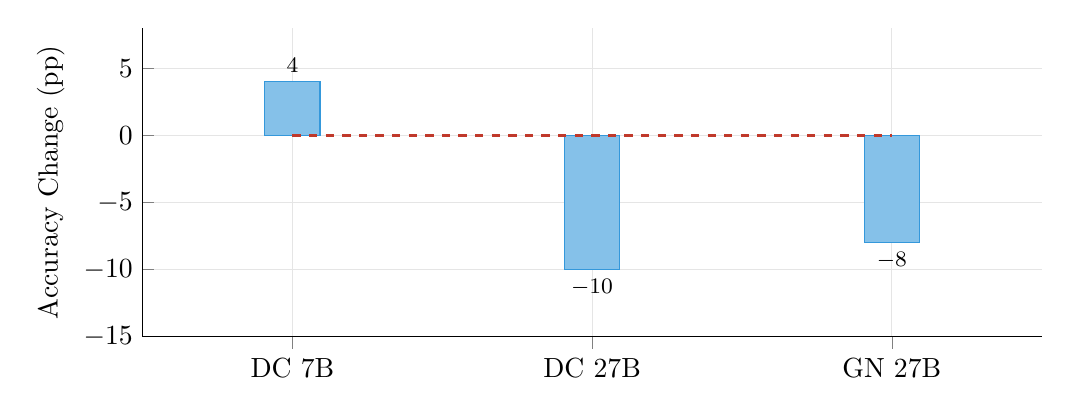
\begin{tikzpicture}
    \begin{axis}[
      ybar,
      width=13cm, height=5.5cm,
      bar width=0.7cm,
      ylabel={Accuracy Change (pp)},
      symbolic x coords={DC 7B, DC 27B, GN 27B},
      xtick=data,
      ymin=-15, ymax=8,
      ytick={-15,-10,-5,0,5},
      grid=major,
      grid style={gray!20},
      nodes near coords,
      every node near coord/.append style={font=\footnotesize},
      axis x line*=bottom,
      axis y line*=left,
      enlarge x limits=0.25,
    ]
      \addplot[fill=niceblue!60, draw=niceblue] coordinates {
        (DC 7B, 4) (DC 27B, -10) (GN 27B, -8)
      };
      \draw[thick, dashed, errorred] (axis cs:DC 7B, 0) -- (axis cs:GN 27B, 0);
    \end{axis}
  \end{tikzpicture}
  \end{center}

  \vspace{0.1cm}

  \begin{columns}[T]
    \begin{column}{0.48\textwidth}
      \begin{alertblock}{Why DQS Fails}
        \begin{enumerate}
          \item Leading questions $\rightarrow$ evasive answers
          \item Fixation on one suspect/digit
          \item Compound questions $\rightarrow$ compound noise
          \item DC-7B ``$+$4pp'' was within noise
        \end{enumerate}
      \end{alertblock}
    \end{column}
    \begin{column}{0.48\textwidth}
      \begin{block}{Implication}
        The bottleneck is \textbf{not} question quality.

        \vspace{0.1cm}

        \textbf{DC:} NPC responses are noise regardless of question.

        \textbf{GN:} Model can't use feedback regardless of guess quality.

        \vspace{0.1cm}

        DQS attacks the wrong bottleneck.
      \end{block}
    \end{column}
  \end{columns}
\end{frame}

%==============================================================================
\section{Key Findings \& Next Steps}
%==============================================================================

\begin{frame}{Week 6 Findings}

  \small
  \begin{enumerate}
    \item \textbf{DQS collapsed: 60\% $\rightarrow$ 29\% at $n{=}100$}
    --- Week 5 headline was a statistical artifact. DQS hurts across all tasks.

    \vspace{0.1cm}

    \item \textbf{Questioning hurts DC --- confirmed across 7B and 27B}
    --- Zero-shot $>$ Fixed(10) for both models. NPC responses are noise.

    \vspace{0.1cm}

    \item \textbf{MI-based stopping works on SP (F1: 0.72 $\rightarrow$ 0.80, $p < 0.001$)}
    --- The one clean positive result. Ground-truth feedback enables systematic elimination.

    \vspace{0.1cm}

    \item \textbf{Gemma-27B breaks GN 0\% barrier: 12\% accuracy}
    --- Dense 27B $>$ 3B-active MoE $>$ 7B. Model scale is the dominant factor.

    \vspace{0.1cm}

    \item \textbf{GN needs max turns --- MI stopping is counterproductive}
    --- min\_turns ablation: 3$\rightarrow$5$\rightarrow$10$\rightarrow$25 maps to 1\%$\rightarrow$2\%$\rightarrow$9\%$\rightarrow$12\%.
  \end{enumerate}
\end{frame}

\begin{frame}{Next Steps}
  \begin{itemize}
    \item \textbf{DC with Gemma-27B + MI/KnowNo} --- does MI add value
          when the base model is stronger (57\% zero-shot)?

    \vspace{0.15cm}

    \item \textbf{SP with Gemma-27B} --- can the stronger model push
          F1 beyond 0.80?

    \vspace{0.15cm}

    \item \textbf{GN with larger dense model} --- Qwen3-Coder full (80B)
          or GPT-4o-mini. If 27B $=$ 12\%, 80B might reach 30\%+.

    \vspace{0.15cm}

    \item \textbf{GN error analysis} --- 31/88 failures hit 3 bulls.
          Can we add a constraint-tracking scaffold to close the last digit?

    \vspace{0.15cm}

    \item \textbf{Variance estimation} --- run each method 3$\times$
          to quantify run-to-run instability.
  \end{itemize}

  \vspace{0.5cm}

  \begin{center}
    \large\textbf{End}
  \end{center}
\end{frame}

\end{document}
